% ---------------------------------------------------------------------------
% Figure captions for the five validation panels.
%
% Style matches the reference caption: bold title, per-subpanel (A)-(D)
% descriptions carrying exact numbers, colours, axis scales, and view angles,
% each clause tied to the theorem it corroborates. Numbers are taken verbatim
% from experiments/results.json and the panel-generation grids.
%
% Cross-references use \Cref{...}; if the main file does not load cleveref,
% replace \Cref with \ref (and supply the leading word, e.g. "Theorem~\ref{...}").
% Colours named below match make_panels.py: steel-blue #1f6feb (high-capability
% / primary), coral #e8710a (regional / secondary / reference line), sea-green
% #2a9d5c (accent), grey #888888 (floor / threshold), viridis (all surfaces).
% ---------------------------------------------------------------------------

\begin{figure*}[!htbp]
    \centering
    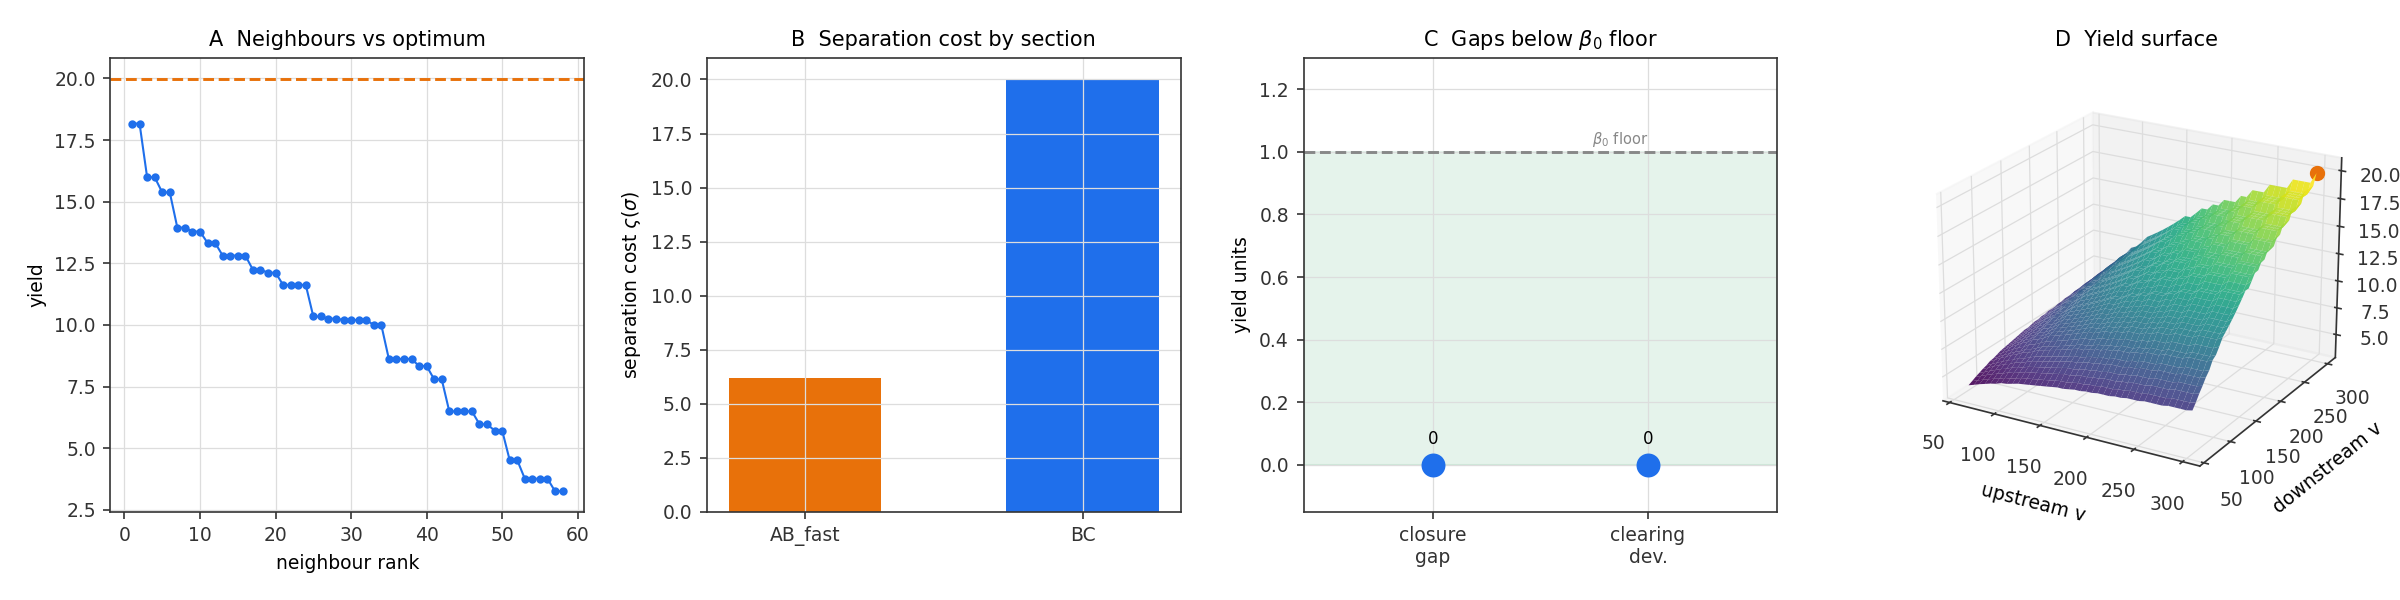
\includegraphics[width=\textwidth]{figures/panel_1_equivalence.png}
    \caption{\textbf{Occupancy--Closure--Clearing Coincide at One Fixed Point.}
    (\textbf{A})~Yield of every task-delivering single-section neighbour of the
    brute-force optimum on the linear $y$-axis, sorted descending against
    neighbour rank ($1$ to $58$) on the linear $x$-axis (steel-blue), with the
    optimum $\yield^\star=19.98$ marked (coral dashed). All $58$ neighbours that
    still deliver the demand lie strictly below the optimum: the best improving
    reassignment gains nothing, so the configuration admits no
    $\blocktime$-improving move and is closed, the empirical content of
    \Cref{thm:trinity}(i)$\Rightarrow$(ii).
    (\textbf{B})~Per-section separation cost $\sep(\sigma)$ on the linear
    $y$-axis for the two sections carrying the flow: the substitutable upstream
    section \texttt{AB\_fast} ($\sep=6.19$, coral) and the essential downstream
    section \texttt{BC} ($\sep=19.98$, steel-blue). The gap between them is the
    quantitative content of \Cref{def:sepcost}: separation cost discriminates a
    bottleneck from a section with a partial substitute, and equals the clearing
    price by construction (\Cref{thm:trinity}(iii)).
    (\textbf{C})~Closure gap and maximum clearing-deviation profit at the
    optimum on the linear $y$-axis (yield units), each plotted as a marker
    (steel-blue) inside the sub-floor band (sea-green shading) beneath the
    resolution floor $\blocktime=1.00$ (grey dashed). Both are exactly $0$: no
    reassignment and no participant deviation gains more than the floor, so
    closure and clearing hold simultaneously, closing the equivalence cycle of
    \Cref{thm:trinity}.
    (\textbf{D})~Three-dimensional yield surface over the upstream-vehicle speed
    ($60$ to $300$~km/h) and downstream-vehicle speed ($60$ to $300$~km/h) at
    the fixed optimal carried set, viridis colourmap, viewing angle elevation
    $22^{\circ}$ azimuth $-60^{\circ}$. The surface rises monotonically toward
    the fast/fast corner where the closed optimum sits (coral marker), showing
    that yield-optimality, closure, and clearing designate the same
    configuration.}
    \label{fig:val_equivalence}
\end{figure*}

\begin{figure*}[!htbp]
    \centering
    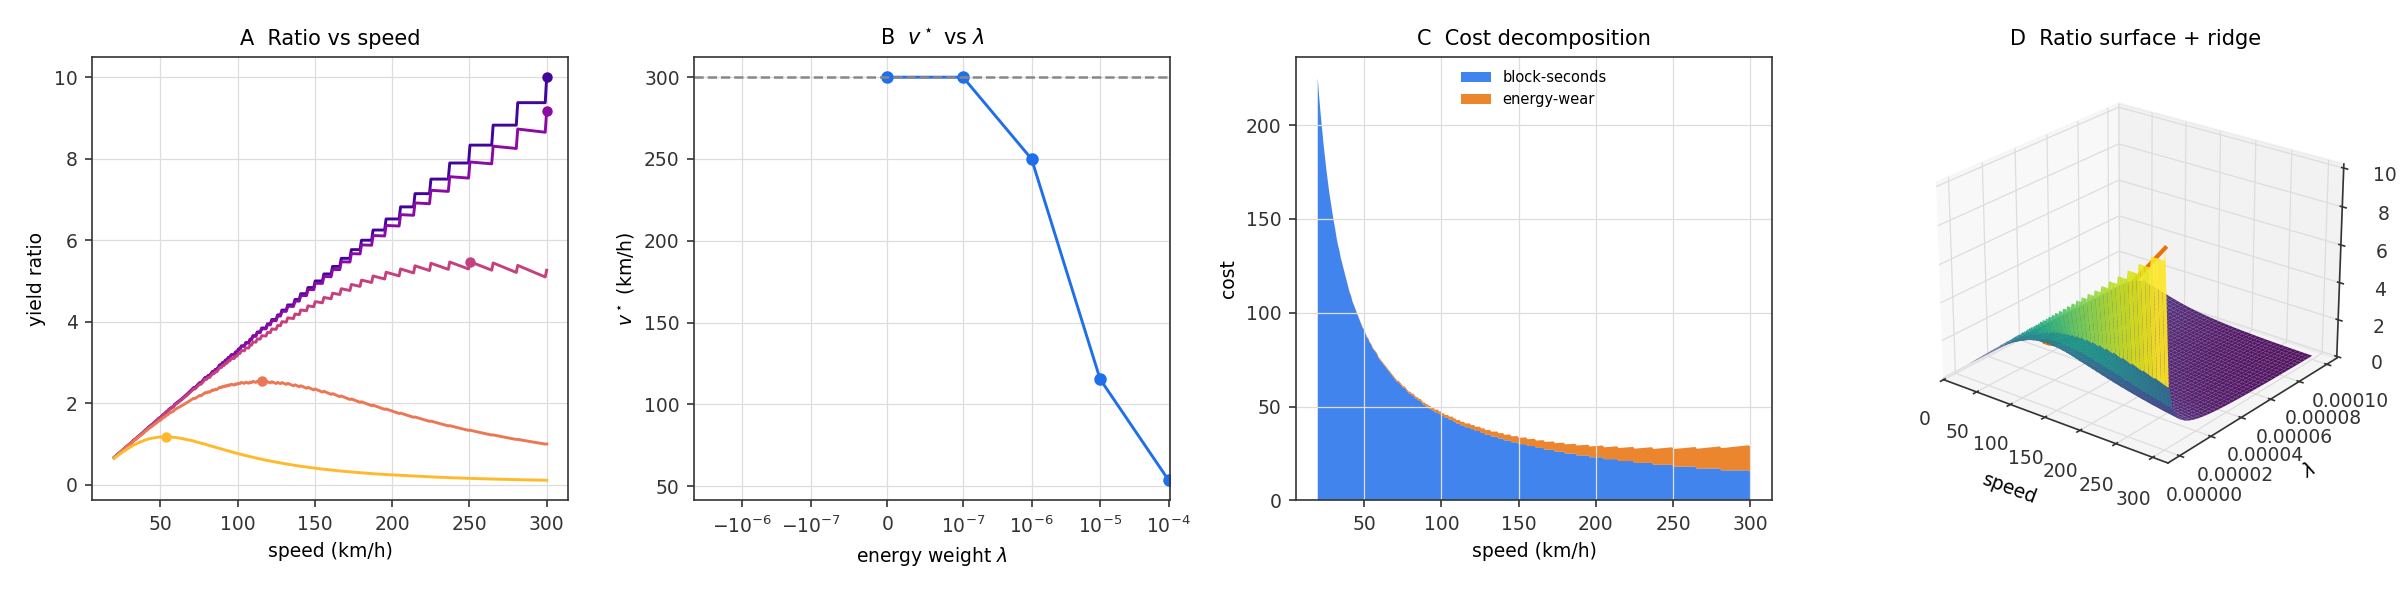
\includegraphics[width=\textwidth]{figures/panel_2_forced_speed.png}
    \caption{\textbf{Optimal Speed Is Forced, Not Imposed.}
    (\textbf{A})~Yield ratio on the linear $y$-axis versus traversal speed
    ($20$ to $300$~km/h) on the linear $x$-axis, one curve per energy weight
    $\lambda\in\{0,10^{-7},10^{-6},10^{-5},10^{-4}\}$ (plasma colour ramp), each
    peak marked. Every curve is single-peaked, and the peak is the
    section-optimal speed $v^\star$ of \Cref{def:optspeed}: for $\lambda=0$ the
    peak sits at the capability ceiling, while for $\lambda=10^{-4}$ it has moved
    well into the interior.
    (\textbf{B})~$v^\star$ on the linear $y$-axis versus energy weight $\lambda$
    on a symmetric-log $x$-axis (linear threshold $10^{-7}$), steel-blue with
    markers, capability ceiling $300$~km/h marked (grey dashed). $v^\star$
    equals the ceiling at $\lambda\le 10^{-7}$ and decreases monotonically
    through $250$, $115.4$, $53.6$~km/h as energy cost binds---the signature of
    the strictly convex energy term and the exact statement of
    \Cref{thm:forcedspeed}.
    (\textbf{C})~Denominator decomposition at $\lambda=10^{-6}$: block-second
    cost (steel-blue) and energy--wear cost (coral) stacked on the linear
    $y$-axis versus speed ($20$ to $300$~km/h). Block-seconds fall with speed
    while energy--wear rises, and the balance point of the two is $v^\star$;
    this is the trade-off whose interior minimiser \Cref{def:optspeed} isolates.
    (\textbf{D})~Three-dimensional yield-ratio surface over speed
    ($20$ to $300$~km/h) and energy weight $\lambda$ ($0$ to $10^{-4}$), viridis
    colourmap, with the ridge of maxima traced (coral), viewing angle elevation
    $24^{\circ}$ azimuth $-52^{\circ}$. The ridge descends from the ceiling into
    the interior as $\lambda$ grows, visualising $v^\star(\lambda)$ as a
    well-defined curve rather than a degenerate ``always maximal.''}
    \label{fig:val_forced_speed}
\end{figure*}

\begin{figure*}[!htbp]
    \centering
    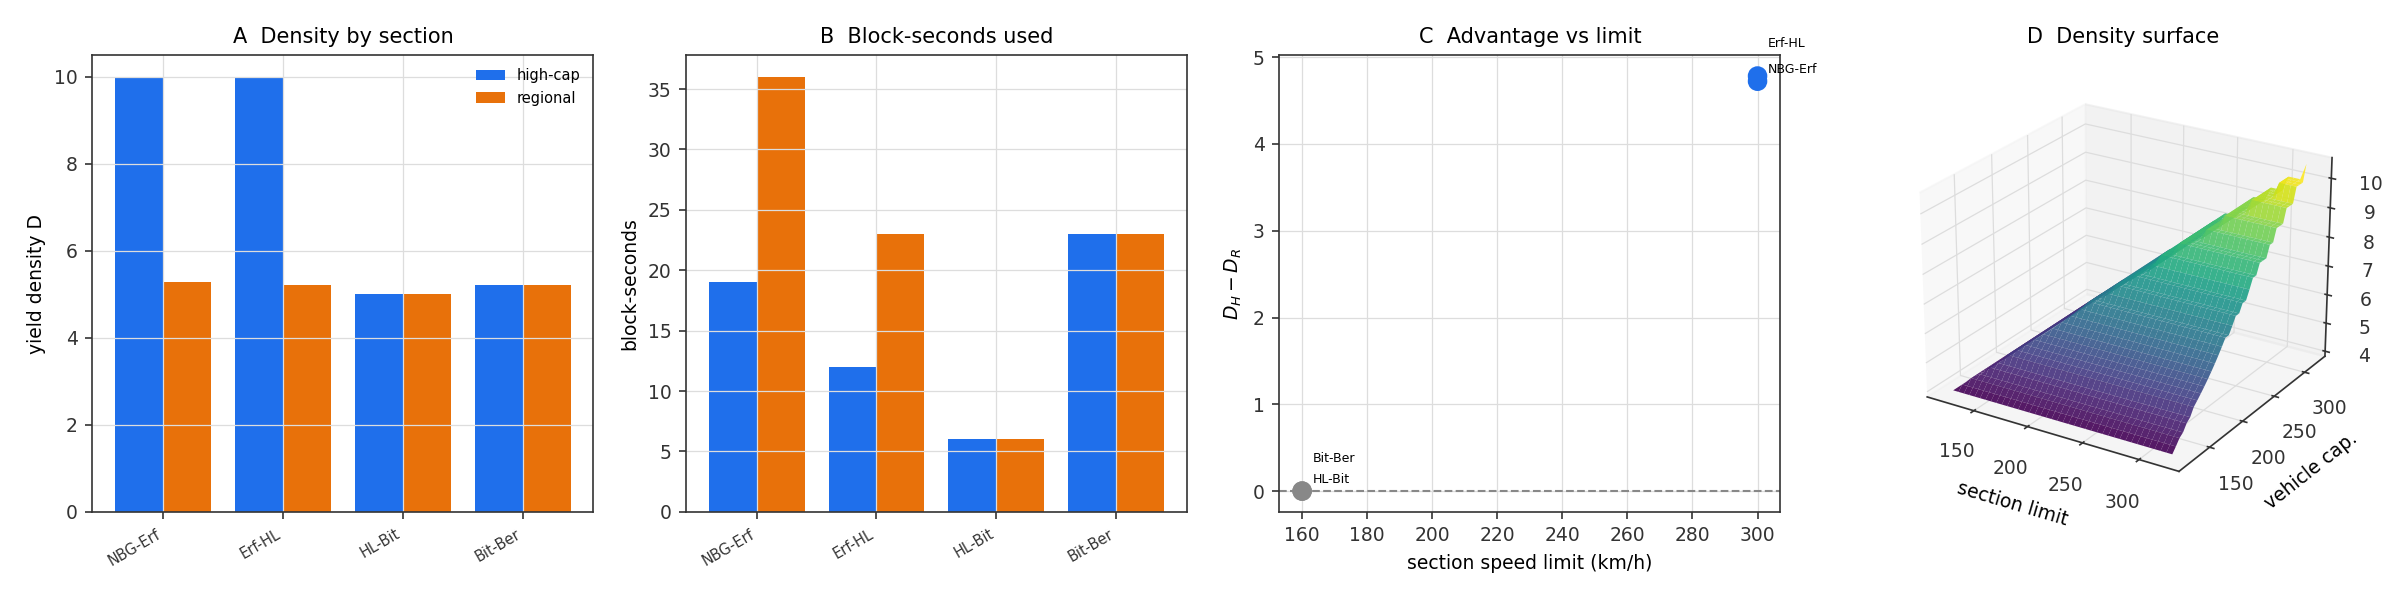
\includegraphics[width=\textwidth]{figures/panel_3_sorting.png}
    \caption{\textbf{The Fleet Sorts Itself by Comparative Advantage.}
    (\textbf{A})~Yield density on the linear $y$-axis for the high-capability
    vehicle (steel-blue) and the regional vehicle (coral) across the four
    Nuremberg--Berlin sections. On the two $300$~km/h new-build sections the
    high-capability vehicle dominates ($D=10.0$ versus $5.28$ and $5.22$); on
    the two $160$~km/h speed-limited sections the densities coincide
    ($5.0$ and $5.22$), the exact content of \Cref{thm:sorting}.
    (\textbf{B})~Block-seconds consumed on the linear $y$-axis by each vehicle
    class per section (high-capability steel-blue, regional coral). The gap on
    the fast sections---$19$ against $36$ block-seconds on \texttt{NBG-Erf}---is
    the resource cost on which the density advantage of panel~A rests; on the
    limited sections the counts match.
    (\textbf{C})~Density advantage $D_H-D_R$ on the linear $y$-axis versus
    section speed limit ($160$ to $300$~km/h) on the linear $x$-axis, one point
    per section, coloured steel-blue where the advantage is positive and grey
    where it vanishes, zero line marked (grey dashed). The advantage is
    ${\approx}4.8$ at $300$~km/h and exactly $0$ at $160$~km/h, crossing to zero
    precisely where the civil limit falls to the regional ceiling.
    (\textbf{D})~Three-dimensional yield-density surface over section speed limit
    ($120$ to $320$~km/h) and vehicle capability ($120$ to $320$~km/h), viridis
    colourmap, viewing angle elevation $24^{\circ}$ azimuth $-58^{\circ}$.
    Density increases with capability only while the section limit exceeds it and
    saturates once the limit binds, so above each section the higher surface
    identifies the winning vehicle---comparative advantage measured in
    block-seconds, as \Cref{thm:sorting} requires.}
    \label{fig:val_sorting}
\end{figure*}

\begin{figure*}[!htbp]
    \centering
    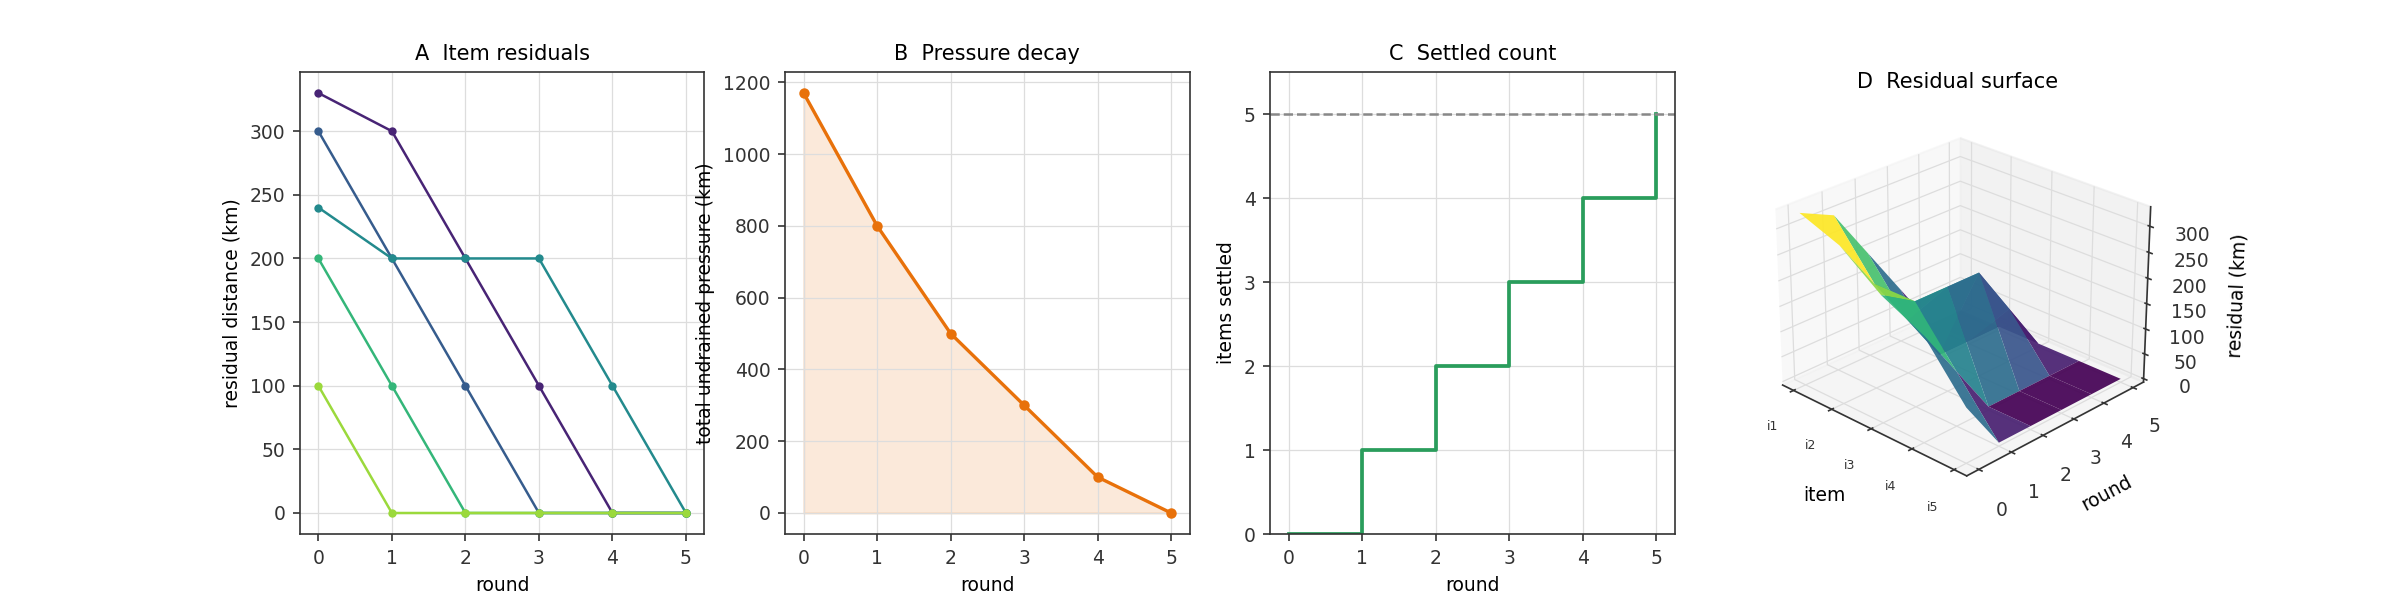
\includegraphics[width=\textwidth]{figures/panel_4_liveness.png}
    \caption{\textbf{Local Descent Drains Every Buffer.}
    (\textbf{A})~Residual distance to target (km) on the linear $y$-axis versus
    routing round ($0$ to $5$) on the linear $x$-axis, one trajectory per item
    for the five items (viridis colour ramp). Every trajectory is monotone
    non-increasing and reaches zero within six rounds, the settling guarantee of
    \Cref{thm:liveness} under greedy target-ward routing (\Cref{def:routing}).
    (\textbf{B})~Total undrained buffer pressure (summed residual distance, km)
    on the linear $y$-axis versus round (coral, shaded to the axis). Pressure
    falls from $1170$~km to $0$ as buffers drain, the decay to the settled state
    predicted by \Cref{thm:liveness}.
    (\textbf{C})~Number of items settled on the linear $y$-axis versus round as a
    step trace (sea-green), full population $5$ marked (grey dashed). The count
    rises monotonically to five by round five: no item is stranded, and the
    directed feeder corridor---not universally gradient-connected but
    target-descendable---satisfies the weaker hypothesis of
    \Cref{rem:target_relative}.
    (\textbf{D})~Three-dimensional surface of residual distance over item index
    (five items) and round ($0$ to $5$), viridis colourmap, viewing angle
    elevation $26^{\circ}$ azimuth $-46^{\circ}$. The surface descends
    everywhere to the zero floor, visualising the simultaneous draining of all
    buffers on a directed corridor and corroborating liveness under exactly the
    target-relative condition of \Cref{rem:target_relative}.}
    \label{fig:val_liveness}
\end{figure*}

\begin{figure*}[!htbp]
    \centering
    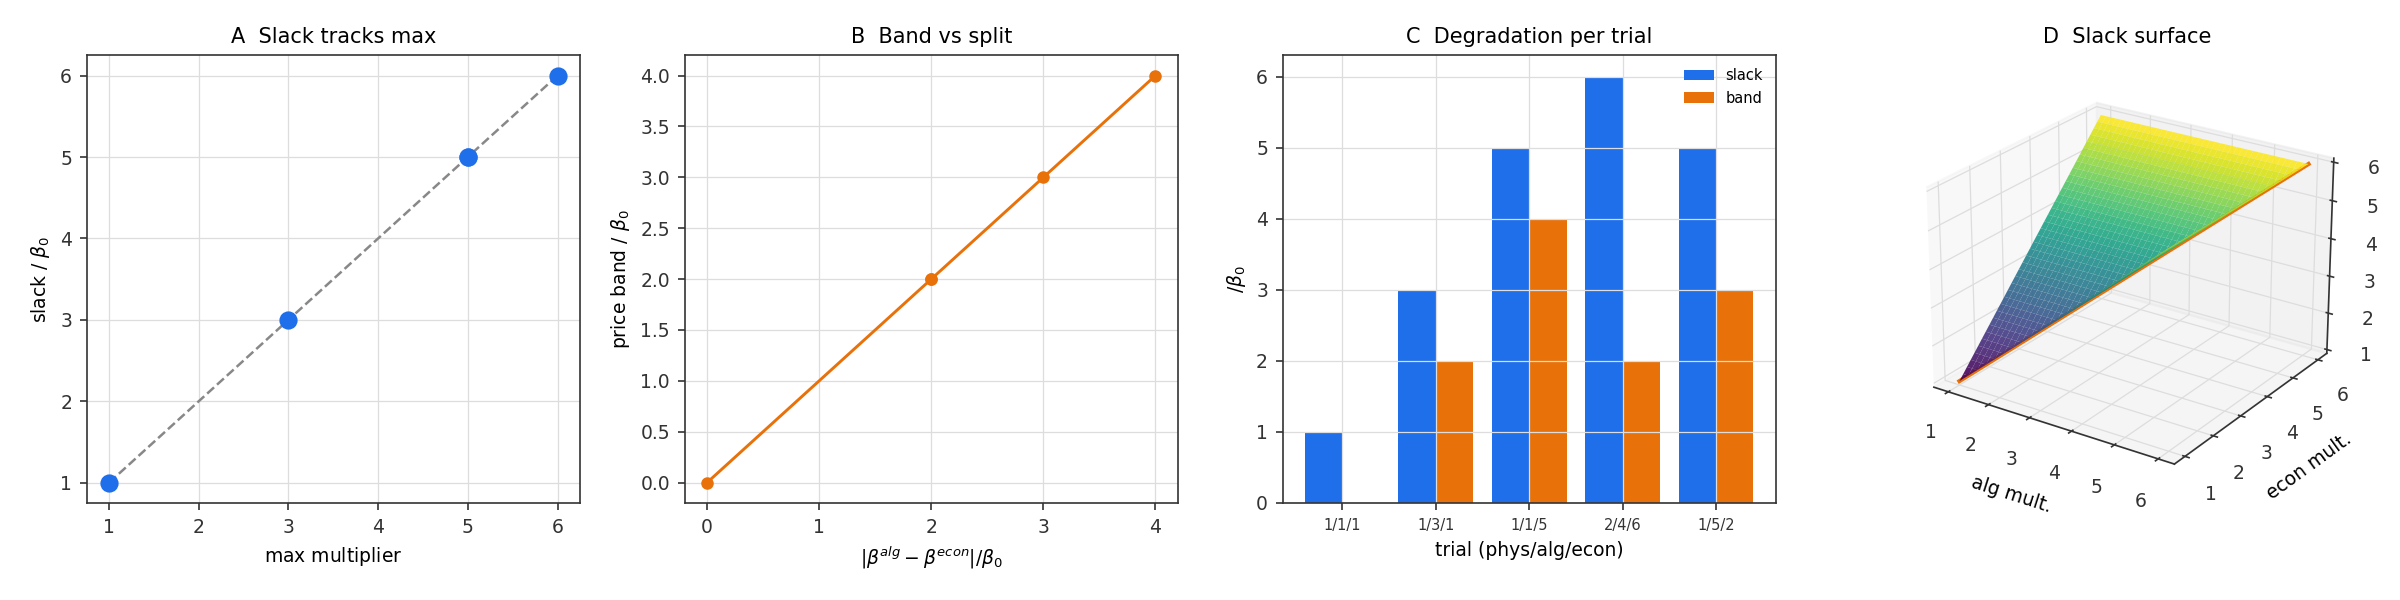
\includegraphics[width=\textwidth]{figures/panel_5_quantum.png}
    \caption{\textbf{The Equivalence Needs One Quantum, Not Three.}
    (\textbf{A})~Equivalence slack in units of $\blocktime$ on the linear
    $y$-axis versus the largest of the three split constants
    (physical/algorithmic/economic multipliers) on the linear $x$-axis, one
    point per trial (steel-blue), identity line marked (grey dashed). The slack
    lies on the diagonal---it equals the maximum of the three constants---and is
    minimal only when all three coincide, the first clause of
    \Cref{prop:quantum}.
    (\textbf{B})~Price-versus-separation band width in units of $\blocktime$ on
    the linear $y$-axis versus the algorithmic--economic split
    $|\blocktime^{\mathrm{alg}}-\blocktime^{\mathrm{econ}}|/\blocktime$ on the
    linear $x$-axis (coral with markers). The band grows linearly from $0$ and
    vanishes exactly at zero split, the second clause of \Cref{prop:quantum}:
    the clearing price equals the separation cost only up to
    $|\blocktime^{\mathrm{alg}}-\blocktime^{\mathrm{econ}}|$.
    (\textbf{C})~Slack (steel-blue) and price band (coral), both in units of
    $\blocktime$, on the linear $y$-axis for five trials labelled by their
    physical/algorithmic/economic multipliers on the $x$-axis. The unified
    trial $1/1/1$ shows slack $1$ and band $0$; every split trial shows enlarged
    slack and a nonzero band, exhibiting where the equivalence survives and where
    it degrades.
    (\textbf{D})~Three-dimensional surface of equivalence slack (units of
    $\blocktime$) over the algorithmic multiplier ($1$ to $6$) and economic
    multiplier ($1$ to $6$) at fixed physical floor, viridis colourmap, with the
    diagonal minimum ridge traced (coral), viewing angle elevation $24^{\circ}$
    azimuth $-56^{\circ}$. The unique minimum runs along the diagonal where the
    two constants are equal, confirming \Cref{prop:quantum}: it is the identity
    of the three roles of $\blocktime$, not its magnitude, that makes the three
    fixed points coincide.}
    \label{fig:val_quantum}
\end{figure*}
